% =============================================
% CAPÍTULO 3: DISEÑO E IMPLEMENTACIÓN
% =============================================

\chapterpage{3}{Diseño e Implementación}
\clearpage
\refstepcounter{chapter}
\addcontentsline{toc}{chapter}{Cap. 3 Diseño e Implementación}

En este capítulo se describe el proceso de diseño e implementación del sistema, desarrollando cada uno de los objetivos específicos del proyecto en el orden en que fueron planteados. Para cada objetivo se presentan las decisiones técnicas tomadas y la justificación que las respalda.




% =============================================
% OE 1: BASE DE DATOS
% =============================================

\section{Desarrollo de la base de datos en PostgreSQL}

Para cumplir con el primer objetivo específico se diseñó e implementó una base de datos relacional en PostgreSQL que centraliza toda la información del sistema: productos, lotes de inventario, usuarios, ventas y mediciones ambientales. Una base de datos relacional organiza la información en tablas vinculadas entre sí mediante referencias, lo que permite consultar datos relacionados de forma eficiente y mantener la consistencia de la información. El esquema resultante comprende \textbf{22 tablas} agrupadas en cinco módulos funcionales, y su evolución a lo largo del desarrollo fue gestionada mediante \textbf{13 archivos de migración} versionados con Alembic.

\subsection{Selección de PostgreSQL}

  Se eligió PostgreSQL como sistema gestor de base de datos por ser la opción
  recomendada por los ecosistemas de las herramientas utilizadas en este proyecto
  y por su amplia adopción en el desarrollo de aplicaciones
  web profesionales. Frente a alternativas como MySQL o SQLite, ofrece una ventaja
  concreta para este sistema.
  
  Esta es, el tipo de dato \textbf{NUMERIC}, que almacena cantidades monetarias
  con precisión exacta, sin los errores de redondeo que presentan los tipos de punto
  flotante al acumular operaciones. En un sistema que calcula totales de ventas y
  maneja precios con decimales, esta precisión es necesaria para garantizar que los
  montos registrados sean exactos.

\subsection{Organización modular del esquema}

Las 22 tablas se dividieron en cinco módulos según el área del negocio que gestionan, de modo que cada módulo tenga una responsabilidad clara y las dependencias entre módulos sean explícitas:

\begin{enumerate}[nosep, itemsep=3pt]
    \item \textbf{Autenticación y control de acceso:} usuarios, roles y permisos.
    \item \textbf{Catálogo de productos:} información de los medicamentos y sus características.
    \item \textbf{Inventario y compras:} lotes, fechas de caducidad y órdenes de abastecimiento.
    \item \textbf{Registro de ventas:} transacciones, pagos y devoluciones.
    \item \textbf{Mediciones del sensor:} lecturas de temperatura y humedad.
\end{enumerate}

Esta separación hace que las tablas de un módulo puedan crecer o modificarse sin impactar innecesariamente a los demás, y permite localizar con facilidad qué parte del esquema es responsable de cada tipo de dato.

\begin{figure}[H]
    \centering
    \fbox{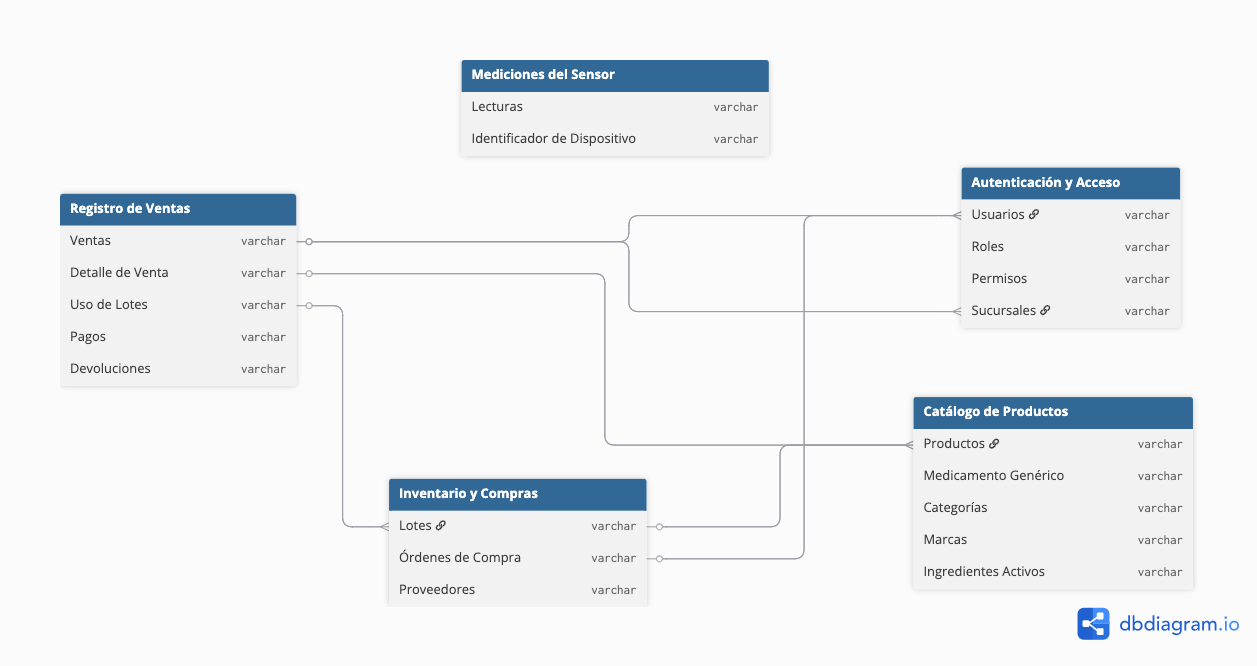
\includegraphics[width=1\textwidth]{0_imagenes/Cap3/DiagramaGeneral.png}}
    \caption{Organización modular de la base de datos y dependencias entre módulos}
    \label{fig:cap3-bd-modulos}
    \vspace{0.2cm}
    \footnotesize \textbf{Fuente:} Elaboración propia.
\end{figure}

\clearpage
\subsection{Módulo 1: Autenticación y control de acceso}

Este módulo agrupa las cinco tablas relacionadas con el acceso al sistema: usuarios, roles, permisos, la relación entre roles y permisos, y sucursales.

El control de acceso se estructuró por roles: cada usuario pertenece a un rol —por ejemplo, \textit{administrador} o \textit{cajero}— y el rol define qué operaciones puede realizar. Esto simplifica la administración: cambiar los privilegios de un grupo de usuarios requiere modificar únicamente el rol, no cada cuenta individualmente.

Para los registros que no deben eliminarse permanentemente —usuarios, roles y sucursales— se optó por conservar el registro en la base de datos y anotar la fecha de baja en una columna adicional. Esto es necesario porque el historial de ventas referencia al usuario que realizó cada transacción; eliminar físicamente ese registro rompería esa relación.

% -------------------------------------------------------
% DIAGRAMA 1 — Módulo de Autenticación y Control de Acceso
% Guardar la imagen generada en dbdiagram.io como:
%   0_imagenes/Cap3/DiagramaAuth.png
% y descomentar el bloque siguiente:
% -------------------------------------------------------
\begin{figure}[H]
    \centering
    \fbox{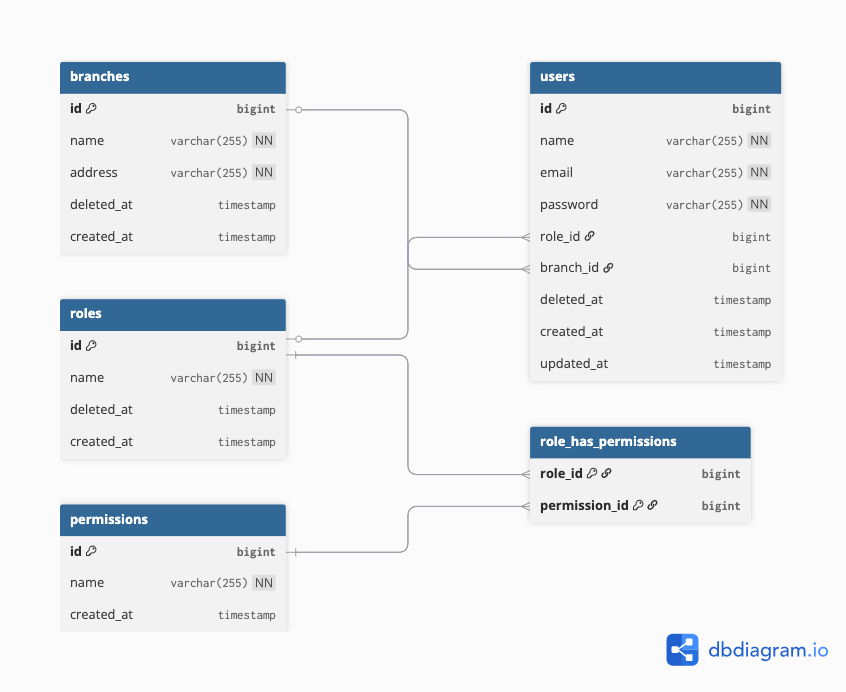
\includegraphics[width=0.8\textwidth]{0_imagenes/Cap3/DiagramaAuth.png}}
    \caption{Diagrama relacional del módulo de autenticación y control de acceso}
    \label{fig:cap3-diagrama-auth}
    \vspace{0.2cm}
    \footnotesize \textbf{Fuente:} Elaboración propia.
\end{figure}

\clearpage
\subsection{Módulo 2: Catálogo de productos}

Este módulo administra la información de los medicamentos mediante seis tablas: \texttt{products}, \texttt{product\_master}, \texttt{product\_categories}, \texttt{product\_brands}, \texttt{ingredients} y \texttt{product\_has\_ingredients}.

Se separó \texttt{product\_master} (medicamento genérico) de \texttt{products} (presentación específica). Por ejemplo, \textit{Paracetamol} es un único registro en \texttt{product\_master}, y sus presentaciones concretas —\textit{Paracetamol 500~mg 20 tabletas}, \textit{Paracetamol suspensión 250~mg/5~ml}— son registros distintos en \texttt{products} que apuntan al mismo genérico. Esto evita duplicar el nombre del principio activo en cada presentación y permite generar reportes agrupados por nombre genérico sin procesamiento adicional.

La tabla \texttt{product\_categories} implementa una \textbf{jerarquía autorelacionada}: la columna \texttt{parent\_id} referencia a la misma tabla, lo que permite representar categorías anidadas (\textit{Medicamentos} → \textit{Analgésicos} → \textit{Antiinflamatorios}) con una única tabla y sin límite fijo de niveles de profundidad.

La tabla \texttt{product\_has\_ingredients} es una tabla de unión que registra qué ingredientes activos contiene cada producto, junto con la cantidad y la unidad de medida (mg, g, ml, UI). Almacenar la composición en la base de datos —en lugar de solo en la etiqueta del producto— hace posible consultar o filtrar medicamentos por principio activo directamente desde el sistema.

% -------------------------------------------------------
% DIAGRAMA 2 — Módulo de Catálogo de Productos
% Guardar como: 0_imagenes/Cap3/DiagramaCatalogo.png
% -------------------------------------------------------
\begin{figure}[H]
    \centering
    \fbox{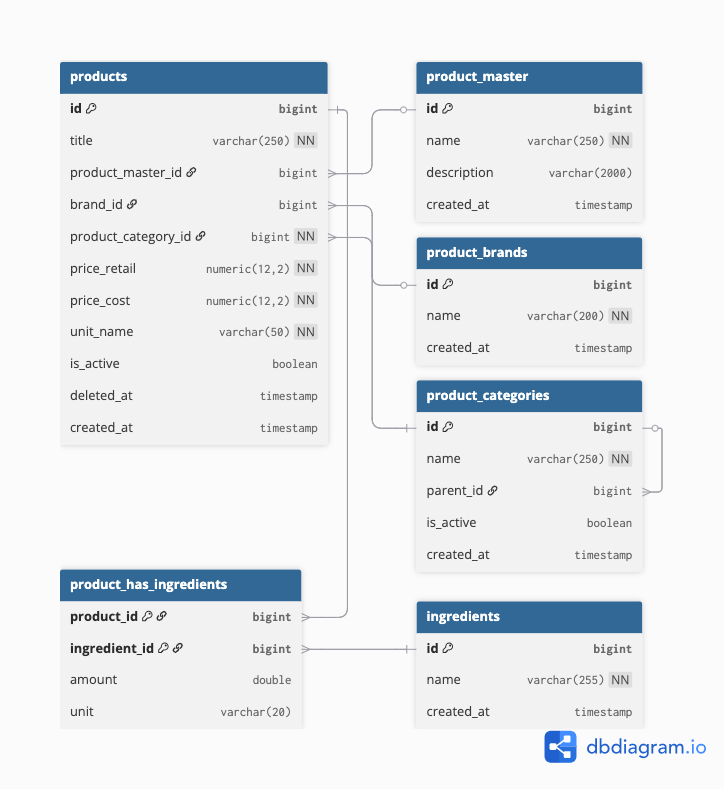
\includegraphics[width=1\textwidth]{0_imagenes/Cap3/DiagramaCatalogo.png}}
    \caption{Diagrama relacional del módulo de catálogo de productos}
    \label{fig:cap3-diagrama-catalogo}
    \vspace{0.2cm}
    \footnotesize \textbf{Fuente:} Elaboración propia.
\end{figure}

\clearpage
\subsection{Módulo 3: Inventario y compras}

Este módulo controla las existencias físicas y el abastecimiento mediante cuatro tablas: \texttt{product\_batches} (lotes), \texttt{suppliers} (proveedores), \texttt{purchases} (órdenes de compra) y \texttt{purchase\_details} (líneas de cada orden).

La tabla central del módulo es \texttt{product\_batches}, que registra cada \textbf{lote} de un producto con su código de lote, fecha de caducidad y cantidad disponible en ese lote. Gestionar el inventario a nivel de lote es técnicamente necesario en una farmacia porque los medicamentos tienen fecha de caducidad por lote, y las regulaciones de buenas prácticas de almacenamiento farmacéutico establecen que deben despacharse primero los lotes que vencen antes, criterio conocido como \textbf{FEFO} (\textit{First Expired, First Out}). Sin este nivel de detalle, el sistema conocería cuántas unidades hay de un producto, pero no podría determinar cuál lote se consumió en cada salida.

Para la columna \texttt{lot\_code} se diseñó un \textbf{índice único parcial} que aplica únicamente cuando el valor no es nulo. Esta restricción resuelve una situación concreta identificada durante el análisis del negocio: algunos medicamentos ingresan a la farmacia sin número de lote asignado por el fabricante. Un índice único convencional rechazaría varias entradas con valor nulo para el mismo producto, impidiendo registrar estos ingresos. El índice parcial permite tantos lotes sin código como sea necesario, pero impide que dos lotes del mismo producto compartan el mismo código no nulo, previniendo registros duplicados por error.

% -------------------------------------------------------
% DIAGRAMA 3 — Módulo de Inventario y Compras
% Guardar como: 0_imagenes/Cap3/DiagramaInventario.png
% -------------------------------------------------------
\begin{figure}[H]
    \centering
    \fbox{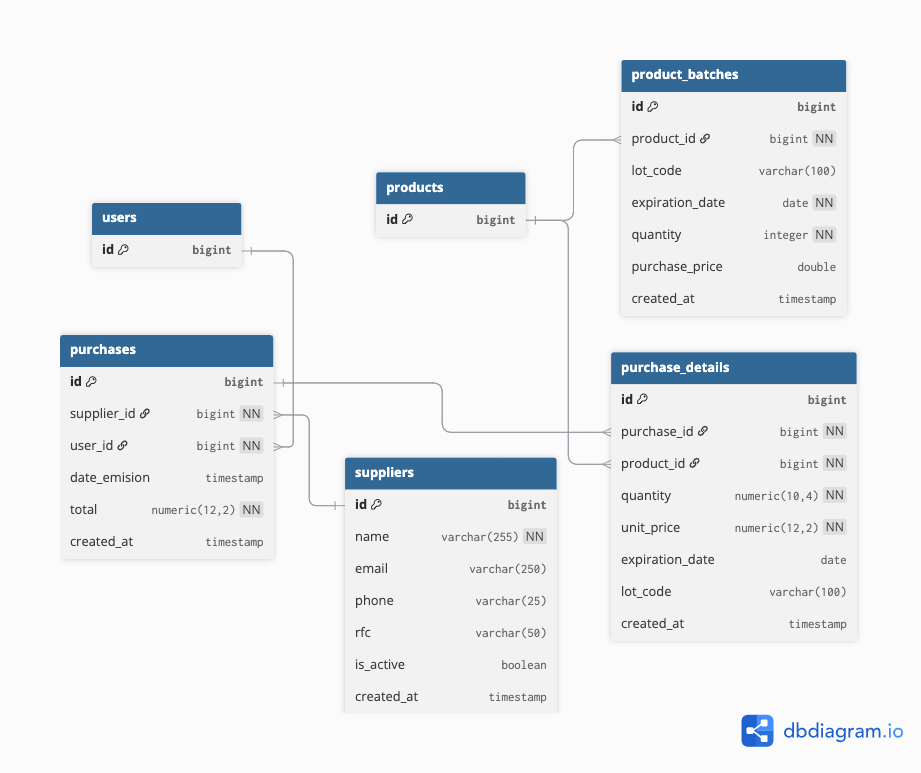
\includegraphics[width=1\textwidth]{0_imagenes/Cap3/DiagramaInventario.png}}
    \caption{Diagrama relacional del módulo de inventario y compras}
    \label{fig:cap3-diagrama-inventario}
    \vspace{0.2cm}
    \footnotesize \textbf{Fuente:} Elaboración propia.
\end{figure}

\clearpage
\subsection{Módulo 4: Registro de ventas}

Este módulo registra las transacciones comerciales mediante cinco tablas: \texttt{sales}, \texttt{sale\_details}, \texttt{sale\_batch\_usage}, \texttt{sale\_payments} y \texttt{refund\_products}.

Se utilizó un diseño de \textbf{cabecera-detalle}: \texttt{sales} almacena los datos generales de cada transacción (empleado que la realizó, sucursal, descuento, impuesto y total), y \texttt{sale\_details} registra cada producto incluido en esa venta con su cantidad y precio unitario. Separar el encabezado de las líneas de detalle permite que una sola venta contenga múltiples productos sin repetir los datos generales en cada línea, y facilita calcular totales agregados con consultas directas a la base de datos.

La tabla \texttt{sale\_batch\_usage} vincula cada línea de venta con el lote específico del que se descontaron las unidades. Esta estructura proporciona \textbf{trazabilidad completa de cada lote}: dado un número de lote, es posible identificar en qué ventas fue despachado. En el contexto farmacéutico, esto resulta necesario ante un retiro de mercado o una alerta sanitaria, ya que permite determinar exactamente qué ventas contienen el lote afectado.

La columna de estado en \texttt{sales} distingue tres situaciones posibles: venta \textbf{en progreso}, \textbf{completada} o \textbf{cancelada}. Mientras la venta está en progreso, el inventario no se descuenta todavía; el descuento ocurre únicamente al confirmar la transacción. Esto evita que una venta incompleta o cancelada descuente existencias de forma prematura.

La tabla \texttt{sale\_payments} se separó de \texttt{sales} para soportar \textbf{pagos divididos}: una misma transacción puede liquidarse con dos métodos de pago distintos —parte en efectivo, parte con tarjeta— registrando cada pago como una fila independiente con su método e importe.

% -------------------------------------------------------
% DIAGRAMA 4 — Módulo de Registro de Ventas
% Guardar como: 0_imagenes/Cap3/DiagramaVentas.png
% -------------------------------------------------------
\begin{figure}[H]
    \centering
    \fbox{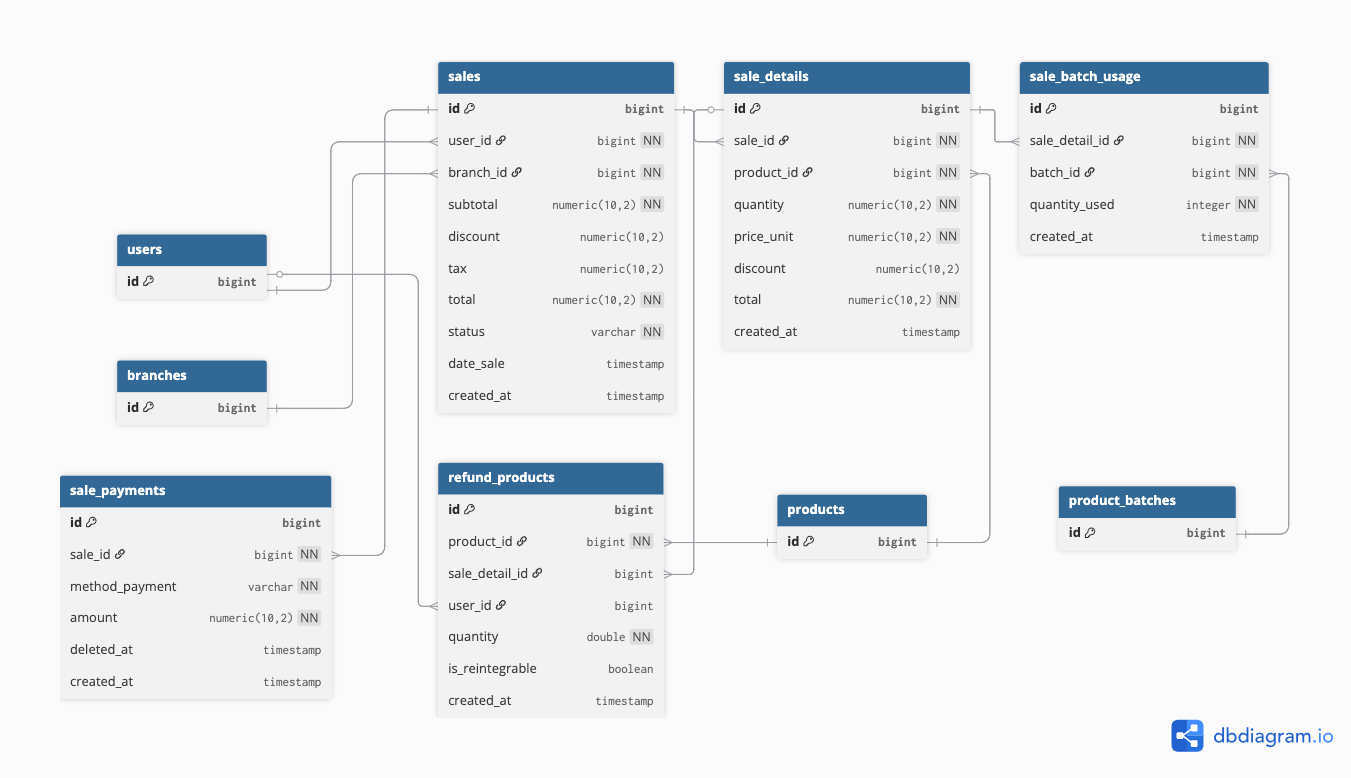
\includegraphics[width=\textwidth]{0_imagenes/Cap3/DiagramaVentas.png}}
    \caption{Diagrama relacional del módulo de registro de ventas}
    \label{fig:cap3-diagrama-ventas}
    \vspace{0.2cm}
    \footnotesize \textbf{Fuente:} Elaboración propia.
\end{figure}

\clearpage
\subsection{Módulo 5: Mediciones del sensor}

Este módulo comprende una sola tabla, \texttt{sensor\_readings}, que almacena cada medición enviada por el nodo electrónico: el valor de temperatura, el valor de humedad, la marca de tiempo en que fue registrada (\texttt{recorded\_at}) y un identificador del dispositivo que la envió (\texttt{device\_id}).

El identificador de dispositivo se definió como cadena de texto en lugar de una llave foránea hacia una tabla de dispositivos, ya que el sistema opera con un único nodo sensor. Crear una tabla de dispositivos completa representaría complejidad estructural sin un beneficio funcional inmediato; el identificador como cadena permite distinguir futuros nodos adicionales sin necesidad de modificar el esquema.

% TODO: subir 0_imagenes/Cap3/DiagramaSensor.png a Overleaf para descomentar
%\begin{figure}[H]
%    \centering
%    \fbox{\includegraphics[width=1\textwidth]{0_imagenes/Cap3/DiagramaSensor.png}}
%    \caption{Diagrama relacional del módulo de mediciones del sensor}
%    \label{fig:cap3-diagrama-sensor}
%    \vspace{0.2cm}
%    \footnotesize \textbf{Fuente:} Elaboración propia.
%\end{figure}

\subsection{Gestión de cambios con Alembic}

El esquema no fue diseñado de forma estática desde el inicio, sino que evolucionó de manera iterativa conforme el desarrollo avanzó y se identificaron ajustes necesarios. Para gestionar esta evolución se utilizó \textbf{Alembic}, una herramienta que actúa como control de versiones para el esquema de la base de datos: cada cambio estructural —crear una tabla, añadir una columna, modificar un tipo de dato— se describe en un archivo de migración numerado que puede aplicarse o revertirse de forma controlada y reproducible.

Se generaron \textbf{13 migraciones} a lo largo del desarrollo. Dos de ellas ilustran el proceso iterativo: la primera fue la conversión de columnas monetarias de \texttt{DOUBLE} a \texttt{NUMERIC}, necesaria tras detectar discrepancias en totales causadas por la aritmética de punto flotante; la segunda fue la adición de \texttt{deleted\_at} a las tablas cuya eliminación física rompería el historial de ventas. Ambos cambios se aplicaron sin pérdida de información ni rediseño del esquema.

El uso de Alembic garantizó además que el entorno de desarrollo local y el entorno de producción desplegado en Railway mantuvieran siempre la misma versión del esquema, eliminando inconsistencias entre ambos entornos.

Con esta estructura, el esquema cubre la totalidad de las entidades descritas en el objetivo: el módulo de autenticación gestiona los usuarios y el control de acceso, el catálogo y el inventario cubren los productos y sus niveles de existencia por lote, el módulo de ventas registra las transacciones comerciales y su trazabilidad, y el módulo de sensor almacena las mediciones ambientales del nodo electrónico.




% =============================================
% OE 2: API REST
% =============================================

\clearpage
\section{Desarrollo de la API REST con FastAPI}

Para cumplir con el segundo objetivo específico se diseñó e implementó una API REST en Python utilizando el \textit{framework} FastAPI. Una API REST es una interfaz de comunicación que permite a los clientes —la aplicación web y el nodo sensor— enviar peticiones HTTP y recibir datos estructurados en formato JSON. La API resultante expone \textbf{23 módulos de rutas} organizados bajo el prefijo \texttt{/api/v1} y gestiona las operaciones de inventario, ventas, usuarios, compras y lecturas del sensor.

\subsection{Selección de FastAPI}

Se eligió FastAPI en lugar de alternativas como Flask o Django REST Framework por tres razones técnicas concretas.

La primera es la \textbf{validación automática de datos de entrada} a través de Pydantic. Cada petición es verificada contra los tipos y restricciones definidos en los esquemas antes de que el código del \textit{endpoint} se ejecute; si un campo obligatorio falta o un valor está fuera de rango, FastAPI devuelve un error descriptivo sin necesidad de código de validación manual.

La segunda es el soporte nativo para \textbf{programación asíncrona} (\texttt{async/await}), que permite al servidor atender múltiples peticiones concurrentes sin bloquear el hilo de ejecución durante las operaciones de entrada/salida —como las consultas a PostgreSQL— mejorando la capacidad de respuesta bajo carga simultánea.

La tercera es la \textbf{generación automática de documentación interactiva} en \texttt{/docs} (estándar OpenAPI), que describe cada \textit{endpoint}, sus parámetros y sus posibles respuestas directamente a partir del código. Esto eliminó la necesidad de mantener documentación separada durante el desarrollo.

\subsection{Arquitectura en capas}

La API se estructuró en capas con responsabilidades distintas: cada petición HTTP desciende por la pila hasta la base de datos y la respuesta asciende por el mismo camino. Esta separación garantiza que los cambios en una capa —por ejemplo, modificar la lógica de negocio o sustituir el motor de base de datos— no requieran modificar las demás.

\begin{figure}[H]
\centering
\begin{tikzpicture}[
    node distance=0.5cm,
    box/.style={rectangle, draw, rounded corners=4pt, minimum width=9.5cm, minimum height=0.82cm, align=center, font=\small},
    arr/.style={Stealth-Stealth, thick, gray!70}
]
\node[box, fill=gray!15]   (client)  {Cliente HTTP \quad (navegador / nodo sensor)};
\node[box, fill=blue!10,   below=of client]  (router)  {Router \quad \texttt{/api/v1/\{recurso\}}};
\node[box, fill=blue!18,   below=of router]  (auth)    {Seguridad — verificación de identidad y permisos};
\node[box, fill=green!10,  below=of auth]    (logic)   {Lógica de negocio — validaciones de dominio y cálculos};
\node[box, fill=orange!10, below=of logic]   (orm)     {Capa de acceso a datos};
\node[box, fill=red!10,    below=of orm]     (db)      {PostgreSQL};
\foreach \a/\b in {client/router, router/auth, auth/logic, logic/orm, orm/db}
    \draw[arr] (\a) -- (\b);
\end{tikzpicture}
\caption{Arquitectura en capas de la API REST}
\label{fig:cap3-api-capas}
\vspace{0.2cm}
\footnotesize \textbf{Fuente:} Elaboración propia.
\end{figure}

El \textbf{enrutador} recibe cada petición y la dirige al componente correcto según la dirección solicitada; la \textbf{capa de seguridad} verifica que el usuario esté identificado y tenga autorización para realizar la operación antes de continuar; la \textbf{lógica de negocio} aplica las reglas del sistema —por ejemplo, comprobar que haya stock suficiente antes de registrar una venta—; la \textbf{capa de acceso a datos} comunica esas operaciones con la base de datos; y \textbf{PostgreSQL} almacena y recupera la información.

\subsection{Modelos ORM con SQLAlchemy}

SQLAlchemy es una biblioteca que implementa el patrón \textbf{ORM} (\textit{Object-Relational Mapping}): en lugar de escribir consultas SQL manualmente en el código, el desarrollador trabaja con clases Python que representan las tablas de la base de datos, y la biblioteca se encarga de traducir esas operaciones al lenguaje de la base de datos. Cada tabla del esquema descrito en el OE1 tiene una clase correspondiente, organizada por módulo.

Este enfoque centraliza la definición de la estructura de datos en un único lugar: cualquier modificación al esquema —agregar una columna o renombrar un campo— se refleja en toda la aplicación sin tener que buscar y actualizar consultas SQL dispersas en el código. Además, al trabajar con tipos definidos en el lenguaje, se reduce la posibilidad de errores de sintaxis o de datos que son difíciles de detectar cuando el SQL se construye manualmente.

\subsection{Esquemas de validación con Pydantic}

Cada módulo define dos tipos de modelos distintos: el \textbf{modelo ORM} para interactuar con la base de datos, y el \textbf{esquema Pydantic} que actúa como un molde o contrato de la API: establece exactamente qué información se acepta cuando el cliente envía datos, qué campos pueden modificarse y qué se devuelve en la respuesta. Si la petición no cumple la forma esperada —por ejemplo, un precio negativo o un campo obligatorio ausente—, Pydantic la rechaza antes de que llegue a la lógica de la aplicación.

Para cada recurso se definieron cuatro esquemas: \texttt{*Base} (campos comunes), \texttt{*Create} (validación al crear), \texttt{*Update} (validación al actualizar) y \texttt{*Response} (estructura de la respuesta). Esta jerarquía evita duplicar definiciones y hace explícito qué datos son públicos y cuáles son internos.


\subsection{Autenticación y autorización}

\subsubsection*{JSON Web Token (JWT): Autenticación y Seguridad}

La autenticación se implementó con \textbf{JWT} (\textit{JSON Web Token}), un estándar que permite emitir credenciales firmadas digitalmente. Al iniciar sesión, la API verifica la contraseña y emite dos elementos: un \textbf{token de acceso} con vigencia de 30 minutos que contiene el identificador del usuario, su rol y sus permisos; y un \textbf{token de renovación} de 7 días almacenado en la base de datos. El token de acceso acompaña cada petición posterior y el servidor lo verifica sin consultar la base de datos, ya que toda la información necesaria está incluida y firmada dentro del propio token. Cuando el token de acceso expira, el cliente usa el token de renovación para obtener uno nuevo sin que el usuario tenga que iniciar sesión de nuevo.


\begin{figure}[H]
\centering
\begin{tikzpicture}[
    node distance=0.5cm and 2.2cm,
    box/.style={rectangle, draw, rounded corners=3pt, minimum width=6.2cm, minimum height=0.82cm, align=center, font=\small},
    dec/.style={diamond, draw, aspect=2.5, align=center, font=\small, inner sep=1pt},
    err/.style={rectangle, draw, rounded corners=3pt, fill=red!10, minimum width=2.4cm, minimum height=0.82cm, align=center, font=\small},
    arr/.style={-{Stealth}, thick}
]
\node[box, fill=gray!15]  (login)   {\textbf{1.} POST /auth/login con credenciales};
\node[box, fill=blue!10,  below=of login]    (verify)  {\textbf{2.} API verifica contraseña (bcrypt)};
\node[dec,                below=of verify]   (valid)   {¿válida?};
\node[box, fill=green!10, below=of valid]    (tokens)  {\textbf{3.} Emitir access token (30 min)\\y refresh token (7 días)};
\node[box, fill=blue!10,  below=of tokens]   (request) {\textbf{4.} Petición enviada con el token de acceso};
\node[dec,                below=of request]  (tokval)  {¿token\\válido?};
\node[box, fill=green!10, below=of tokval]   (exec)    {\textbf{5.} Ejecutar endpoint → respuesta JSON};
\node[err, right=of valid]    (err1) {HTTP 401\\Unauthorized};
\node[err, right=of tokval]   (err2) {HTTP 401\\Token inválido};
\draw[arr] (login) -- (verify);
\draw[arr] (verify) -- (valid);
\draw[arr] (valid) -- node[left, font=\footnotesize]{Sí} (tokens);
\draw[arr] (valid) -- node[above, font=\footnotesize]{No} (err1);
\draw[arr] (tokens) -- (request);
\draw[arr] (request) -- (tokval);
\draw[arr] (tokval) -- node[left, font=\footnotesize]{Sí} (exec);
\draw[arr] (tokval) -- node[above, font=\footnotesize]{No} (err2);
\end{tikzpicture}
\caption{Diagrama de flujo de autenticación mediante JWT}
\label{fig:cap3-jwt-flujo}
\vspace{0.2cm}
\footnotesize \textbf{Fuente:} Elaboración propia.
\end{figure}

\subsubsection*{Control de acceso basado en permisos}

Para la autorización, cada ruta de la API declara explícitamente qué permiso necesita el usuario para acceder a ella. Antes de ejecutar cualquier operación, la API verifica que el token del usuario incluya ese permiso; si no lo tiene, la petición es rechazada sin procesarse. Este mecanismo se apoya directamente en la estructura de roles y permisos definida en la base de datos (OE1): un usuario con rol de cajero solo puede consultar y registrar ventas, mientras que un administrador puede gestionar usuarios, productos y sucursales.

\subsection{Endpoints por módulo}

Un \textit{endpoint} es una dirección específica dentro de la API a la que los clientes envían peticiones para realizar una operación concreta, como consultar el inventario, registrar una venta o actualizar un producto. Cada endpoint combina una URL y un tipo de acción: consulta, creación, actualización o eliminación.

Los 23 módulos de rutas se agrupan en seis áreas funcionales. La siguiente tabla resume la estructura y las operaciones principales de cada grupo:

\begin{table}[H]
\centering
\caption{Agrupación de endpoints de la API REST por área funcional}
\label{tab:cap3-endpoints}
\begin{spacing}{1.0}
\renewcommand{\arraystretch}{1.2}
\begin{tabularx}{\textwidth}{@{}l >{\raggedright}p{3.8cm} X@{}}
\toprule
\textbf{Área} & \textbf{Módulos} & \textbf{Operaciones principales} \\
\midrule
Autenticación      & \texttt{auth}                                                             & Login, emisión y renovación de tokens, cierre de sesión, restablecimiento de contraseña \\[4pt]
Usuarios y acceso  & \texttt{users, roles, permissions, branches}                              & CRUD de usuarios, asignación de roles, gestión de permisos y sucursales \\[4pt]
Catálogo           & \texttt{products, product\_master, categories, brands, ingredients}        & CRUD de medicamentos, jerarquía de categorías, ingredientes activos \\[4pt]
Inventario         & \texttt{product\_batch, suppliers, purchases, purchase\_details}           & Registro de lotes con fechas de caducidad, órdenes de compra \\[4pt]
Ventas             & \texttt{sales, sale\_details, sale\_payments, sale\_batch\_usage, refunds} & Registro de ventas con descuento FEFO, pagos divididos, devoluciones \\[4pt]
Monitoreo          & \texttt{sensor\_readings, dashboard, stats, calendar}                     & Lecturas del sensor, indicadores del negocio, estadísticas \\
\bottomrule
\end{tabularx}
\end{spacing}
\vspace{0.2cm}
\footnotesize \textbf{Fuente:} Elaboración propia.
\end{table}

Todos los \textit{endpoints} siguen las convenciones REST: \texttt{GET} para lectura, \texttt{POST} para creación, \texttt{PUT}/\texttt{PATCH} para actualización y \texttt{DELETE} para eliminación. Los recursos con \texttt{deleted\_at} —usuarios, sucursales, roles— aplican borrado lógico, como se describió en el OE1.

\subsection{Pruebas con Pytest}

La API se verificó mediante dos mecanismos complementarios. El primero es \textbf{Swagger}, la documentación interactiva generada automáticamente por FastAPI en la dirección \texttt{/docs}, que permite enviar peticiones reales a cada \textit{endpoint} directamente desde el navegador y observar las respuestas. Esto facilitó la verificación manual durante el desarrollo sin necesidad de herramientas externas.

El segundo es una suite de pruebas automatizadas con \textbf{Pytest}, compuesta por \textbf{20 archivos de prueba}, uno por cada módulo funcional. Cada prueba verifica que el endpoint responde con el resultado esperado y que las operaciones críticas —como el registro de ventas, el descuento de inventario y el procesamiento de devoluciones— producen resultados correctos. Las pruebas se ejecutan sobre una base de datos de prueba independiente para no interferir con los datos reales.

\subsection{Despliegue en Railway}

La API se desplegó en \textbf{Railway}, una plataforma de infraestructura en la nube que provisiona tanto el servidor de aplicación como la base de datos PostgreSQL en el mismo entorno. Se evaluaron otras opciones como AWS o servidores dedicados, pero resultaban sobredimensionadas para un sistema con una sola instalación activa: Railway ofrece los mismos componentes esenciales a un costo significativamente menor y sin la complejidad de configuración que implica una infraestructura de mayor escala.

Railway se integra directamente con el repositorio de código: cada vez que se publica una nueva versión, el despliegue se actualiza de forma automática. Antes de recibir tráfico, la plataforma ejecuta las migraciones de base de datos pendientes, garantizando que el esquema y el código sean siempre consistentes entre sí.

La información sensible —credenciales de la base de datos, clave de seguridad y parámetros de configuración del entorno— se define como variables en la plataforma, separadas del código fuente, siguiendo la práctica estándar de no incluir datos sensibles en el repositorio.



% =============================================
% OE 3: FRONTEND REACT
% =============================================

\clearpage
\section{Desarrollo de la interfaz web con React}

Para cumplir con el tercer objetivo específico se diseñó e implementó la interfaz de usuario como una \textbf{aplicación web de página única} (\textit{Single Page Application}, SPA): una vez cargada en el navegador, las transiciones entre vistas ocurren sin recargar completamente la página, lo que mejora la fluidez de la experiencia para el usuario. La interfaz se comunica con la API desarrollada en el OE2 para consultar y registrar información. El resultado es una aplicación con \textbf{dieciséis módulos de navegación} cubiertos por una biblioteca de más de cuarenta componentes de interfaz reutilizables, desplegada en la plataforma Vercel.

\subsection{Selección de React y Vite}

Se eligió \textbf{React} como biblioteca base para la construcción de la interfaz por dos razones principales. La primera es su modelo basado en \textbf{componentes reutilizables}: cada elemento visual —una tabla, un formulario, un botón de acción— se define una vez y puede utilizarse en cualquier módulo sin reescribir código. Esto fue determinante dado que la aplicación comparte patrones visuales casi idénticos entre módulos: la estructura de lista con filtros, el formulario de creación y el diálogo de confirmación de eliminación se repiten en inventario, ventas, catálogo y usuarios. La segunda razón es la amplitud de su ecosistema: bibliotecas para gestión de formularios, caché de datos, animaciones y exportación de documentos existen, están mantenidas activamente y se integran entre sí, evitando desarrollar estas funcionalidades desde cero.

Junto con React se utilizó \textbf{Vite} como herramienta de construcción y servidor de desarrollo. Vite moderniza el proceso al servir los módulos directamente al navegador sin reempaquetar todo el proyecto en cada cambio, reduciendo el tiempo entre guardar una modificación y verla reflejada en pantalla. Esto aceleró el ciclo de desarrollo durante la etapa de diseño de la interfaz.

\subsection{Estructura de la aplicación}

La aplicación se organizó en tres niveles de granularidad. Las \textbf{páginas} son los puntos de entrada de cada ruta; las \textbf{secciones} contienen la lógica y la disposición visual específica de cada módulo de negocio; y los \textbf{componentes} son los bloques visuales reutilizables que las secciones ensamblan. El enrutamiento entre páginas se gestiona con \textbf{React Router}, que mapea cada URL a su vista correspondiente sin recargar el servidor. La navegación se realiza desde una barra lateral persistente que agrupa los módulos por área funcional.

El siguiente diagrama resume el flujo general de interacción del usuario con la aplicación, desde el acceso hasta la confirmación de una operación:

\begin{figure}[H]
\centering
\begin{tikzpicture}[
    node distance=0.5cm,
    box/.style={rectangle, draw, rounded corners=3pt, minimum width=8.2cm, minimum height=0.82cm, align=center, font=\small},
    dec/.style={diamond, draw, aspect=2.5, align=center, font=\small, inner sep=1pt},
    err/.style={rectangle, draw, rounded corners=3pt, fill=red!10, minimum width=2.7cm, minimum height=0.82cm, align=center, font=\small},
    arr/.style={-{Stealth}, thick}
]
\node[box, fill=gray!15]  (login)   {\textbf{1.} Pantalla de inicio de sesión};
\node[box, fill=blue!8,   below=of login]   (jwt)    {\textbf{2.} Verificación de credenciales con la API};
\node[dec,                below=of jwt]     (valid)  {¿Válidas?};
\node[err,                right=of valid]   (err)    {Mensaje de\\error al usuario};
\node[box, fill=blue!12,  below=of valid]   (dash)   {\textbf{3.} Panel principal: ventas del día, alertas de stock y sensor};
\node[box, fill=gray!10,  below=of dash]    (nav)    {\textbf{4.} Selección de módulo desde la barra lateral};
\node[box, fill=blue!8,   below=of nav]     (list)   {\textbf{5.} Vista de lista con búsqueda, filtros y paginación};
\node[box, fill=gray!10,  below=of list]    (action) {\textbf{6.} Seleccionar operación: crear, editar o eliminar};
\node[box, fill=blue!8,   below=of action]  (form)   {\textbf{7.} Formulario con validación de datos en el cliente};
\node[dec,                below=of form]    (formv)  {¿Datos\\válidos?};
\node[err,                right=of formv]   (formerr){Indicadores de\\error por campo};
\node[box, fill=green!10, below=of formv]   (api)    {\textbf{8.} Envío a la API y respuesta del servidor};
\node[box, fill=green!8,  below=of api]     (update) {\textbf{9.} Notificación de éxito y actualización automática de la vista};
\draw[arr] (login)  -- (jwt);
\draw[arr] (jwt)    -- (valid);
\draw[arr] (valid)  -- node[left,  font=\footnotesize]{Sí} (dash);
\draw[arr] (valid)  -- node[above, font=\footnotesize]{No} (err);

\draw[arr] (dash)   -- (nav);
\draw[arr] (nav)    -- (list);
\draw[arr] (list)   -- (action);
\draw[arr] (action) -- (form);
\draw[arr] (form)   -- (formv);
\draw[arr] (formv)  -- node[left,  font=\footnotesize]{Sí} (api);
\draw[arr] (formv)  -- node[above, font=\footnotesize]{No} (formerr);
\draw[arr] (api)    -- (update);
\end{tikzpicture}
\caption{Diagrama de flujo general de interacción del usuario con la aplicación web}
\label{fig:cap3-frontend-flujo}
\vspace{0.2cm}
\footnotesize \textbf{Fuente:} Elaboración propia.
\end{figure}

\subsection{Componentes visuales con Material-UI}

Para el diseño visual se eligió \textbf{Material-UI} (MUI), una biblioteca que proporciona un conjunto de componentes construidos sobre las guías de diseño Material Design de Google. La razón principal fue evitar diseñar desde cero elementos como tablas paginadas, formularios, diálogos de confirmación y selectores de fecha, que de otro modo habrían requerido semanas de desarrollo adicional. MUI ofrece estos componentes con comportamiento accesible, adaptación a distintos tamaños de pantalla y un sistema de temas que permite ajustar colores y tipografía de forma centralizada para toda la aplicación.

Para las vistas que muestran listados de registros —productos, lotes, ventas, usuarios— se utilizó el componente de tabla avanzada de MUI, que soporta ordenamiento, filtrado por columna y paginación sin configuración adicional. Dado el volumen moderado de registros que maneja una farmacia de pequeña escala, ordenar y filtrar los datos directamente en la vista es suficiente y evita peticiones adicionales al servidor para cada cambio de orden o filtro.

\subsection{Gestión de datos y estado}

La gestión del estado se dividió en dos responsabilidades distintas. El \textbf{estado de sesión} —la información del usuario autenticado, su rol y sus permisos— se almacena en un contexto global accesible desde cualquier componente. Este estado es necesario para decidir qué secciones del menú mostrar y qué operaciones están disponibles según el rol del usuario activo.

El \textbf{estado de los datos del servidor} —listas de productos, ventas, lotes y demás registros— se gestiona con una biblioteca de caché del lado del cliente. Esta biblioteca conserva en memoria los datos ya consultados; al navegar entre módulos, la información previamente cargada se muestra de inmediato mientras se verifica en segundo plano si hay actualizaciones. Cuando se completa una operación —crear, editar o eliminar un registro—, la vista se refresca automáticamente sin que el usuario tenga que recargar la página. Esta separación entre estado de sesión y estado de datos evitó la necesidad de una solución de gestión de estado global más compleja, cuya configuración no se justifica para una aplicación de esta escala.

\subsection{Formularios y validación}

Todos los formularios de creación y edición se implementaron con \textbf{React Hook Form}, una biblioteca que gestiona el estado del formulario sin causar un re-renderizado completo del componente en cada pulsación de tecla. El beneficio principal es el rendimiento: en formularios con muchos campos —como el registro de ventas con múltiples productos o el alta de un medicamento con ingredientes— la interfaz responde de forma fluida incluso en equipos con recursos limitados.

La validación de cada campo se define mediante esquemas que especifican el tipo de dato esperado, los rangos permitidos y los mensajes de error correspondientes. Esta validación se ejecuta \textit{antes} de enviar la petición a la API, evitando peticiones innecesarias cuando el usuario omite un campo obligatorio o introduce un valor fuera de rango. Los esquemas de validación del cliente se diseñaron para reflejar las mismas restricciones que los esquemas Pydantic definidos en la API (OE2), de modo que las reglas sean consistentes en ambas capas.

Para mantener la consistencia visual y evitar duplicar código, se construyó una biblioteca interna de \textbf{componentes de formulario reutilizables}: campos de texto, selectores, autocompletados con búsqueda, selectores de fecha y casillas de verificación. Cada componente integra la lógica de validación y el estilo de MUI, y puede utilizarse en cualquier formulario de la aplicación conectándolo al esquema de validación correspondiente.

\subsection{Autenticación en el cliente}

Al iniciar sesión, la aplicación recibe los tokens generados por la API (OE2) y los almacena en el navegador: el token de acceso en el almacenamiento de sesión —que se elimina automáticamente cuando el usuario cierra la pestaña o el navegador—, y el token de renovación en el almacenamiento persistente, únicamente cuando el usuario activa la opción de recordar la sesión.

El token de acceso acompaña cada petición a la API. Cuando expira, la aplicación utiliza el token de renovación para obtener uno nuevo de forma transparente, sin interrumpir la sesión. Este mecanismo se implementó en la capa de comunicación HTTP de forma centralizada, de modo que todos los módulos se benefician de él sin código adicional en cada vista.

Las rutas de la aplicación están protegidas mediante \textbf{guardias de acceso}: si el usuario no tiene sesión activa, cualquier intento de acceder a una página del sistema lo redirige a la pantalla de inicio de sesión. Para operaciones que requieren permisos específicos —gestión de usuarios, modificación de roles— el guardia verifica además que los permisos del token incluyan los requeridos, consistente con el módulo RBAC definido en el OE1.

\subsection{Despliegue en Vercel}

La aplicación web se desplegó en \textbf{Vercel}, una plataforma especializada en el alojamiento de aplicaciones JavaScript modernas. Al igual que con Railway para la API, se eligió Vercel sobre alternativas como AWS por la misma razón de escala: ofrece los componentes necesarios —red de distribución de contenido, integración con el repositorio y despliegue automático en cada actualización— sin la complejidad de configuración que implica una infraestructura de mayor tamaño.

Un aspecto particular del despliegue de una SPA es el enrutamiento: dado que React Router gestiona las rutas completamente en el cliente, el servidor de Vercel debe redirigir cualquier URL al punto de entrada de la aplicación para que sea React quien determine qué vista mostrar. Sin esta configuración, acceder directamente a una URL como \texttt{/dashboard/product} devolvería un error del servidor. La redirección se definió en el archivo de configuración de Vercel y garantiza que el usuario pueda acceder a cualquier ruta o recargar la página sin errores.

Las variables de configuración —principalmente la URL de la API— se definen en la plataforma de forma separada al código fuente, siguiendo el mismo criterio de seguridad aplicado en el despliegue de la API.



% =============================================
% OE 4: NODO SENSOR ESP32
% =============================================

\clearpage
\section{Desarrollo del nodo sensor con ESP32}

Para cumplir con el cuarto objetivo específico se diseñó e implementó un nodo electrónico de monitoreo ambiental que mide temperatura y humedad relativa dentro del área de almacenamiento de la farmacia y envía esas lecturas a la API desarrollada en el OE2. El nodo está construido sobre un microcontrolador \textbf{ESP32-C5} con un sensor \textbf{AHT10}, y su firmware fue programado en C++ utilizando el entorno de desarrollo Arduino.

\subsection{Selección del hardware}

\subsubsection*{Microcontrolador ESP32-C5}

Se eligió el \textbf{ESP32-C5} como microcontrolador principal por tres razones. La primera es que integra conectividad \textbf{WiFi 802.11} de forma nativa, sin necesidad de un módulo adicional, lo que simplifica el diseño físico del nodo y reduce su costo. La segunda es que soporta el protocolo de comunicación \textbf{I\textsuperscript{2}C}, necesario para leer el sensor de temperatura y humedad. La tercera es su compatibilidad con el entorno Arduino, que proporciona un ecosistema de bibliotecas maduro para tareas de red, manejo de JSON y gestión de credenciales, reduciendo significativamente el tiempo de desarrollo.

Se descartaron alternativas como un Arduino Uno porque carece de conectividad WiFi integrada, lo que habría requerido un módulo externo y aumentado la complejidad del circuito. Una Raspberry Pi habría sido sobredimensionada para una tarea de lectura y envío periódico de dos valores numéricos, con un consumo de energía y costo mayores sin un beneficio funcional correspondiente.

\subsubsection*{Sensor AHT10}

El \textbf{AHT10} es un sensor que mide simultáneamente temperatura y humedad relativa en un único componente. Se eligió sobre alternativas como los sensores DHT11 o DHT22 por dos motivos. El primero es su protocolo de comunicación: el AHT10 utiliza I\textsuperscript{2}C, un bus estándar de dos hilos (datos y reloj) que es intrínsecamente más robusto ante interferencias que el protocolo de un solo hilo de los sensores DHT. El segundo es su precisión: el AHT10 ofrece una resolución de 0.01 °C en temperatura y 0.024\% en humedad, adecuada para detectar variaciones ambientales relevantes para el almacenamiento farmacéutico, donde rangos como 15–25 °C y 30–65\% de humedad relativa son críticos para la conservación de medicamentos.

\subsection{Arquitectura del firmware}

El firmware sigue el modelo de ejecución de Arduino, que divide el programa en dos funciones con responsabilidades distintas: \textbf{configuración inicial} (\textit{setup}), que se ejecuta una sola vez al encender el dispositivo e inicializa el hardware y la conexión de red; y \textbf{ciclo operativo} (\textit{loop}), que se ejecuta de forma continua y realiza las lecturas periódicas del sensor y el envío de datos.

El diagrama siguiente muestra el flujo completo de ejecución del firmware, desde el encendido hasta el ciclo de operación continua:

\begin{figure}[H]
\centering
\begin{tikzpicture}[
    node distance=0.5cm,
    box/.style={rectangle, draw, rounded corners=3pt, minimum width=8.2cm, minimum height=0.82cm, align=center, font=\small},
    dec/.style={diamond, draw, aspect=2.5, align=center, font=\small, inner sep=1pt},
    err/.style={rectangle, draw, rounded corners=3pt, fill=red!10, minimum width=2.7cm, minimum height=0.82cm, align=center, font=\small},
    warn/.style={rectangle, draw, rounded corners=3pt, fill=orange!10, minimum width=2.7cm, minimum height=0.82cm, align=center, font=\small},
    arr/.style={-{Stealth}, thick}
]
\node[box, fill=gray!15]  (ini)   {\textbf{1.} Encendido del nodo sensor};
\node[box, fill=blue!8,   below=of ini]   (hw)    {\textbf{2.} Inicializar bus I\textsuperscript{2}C y detectar sensor AHT10};
\node[dec,                below=of hw]    (sdet)  {¿Sensor\\detectado?};
\node[err,                right=of sdet]  (errs)  {Error de hardware\\(espera indefinida)};
\node[box, fill=blue!8,   below=of sdet]  (wifi)  {\textbf{3.} Conectar a WiFi mediante portal de provisión};
\node[dec,                below=of wifi]  (wcon)  {¿Conectado?};
\node[err,                right=of wcon]  (errw)  {Reiniciar\\dispositivo};
\node[box, fill=gray!10,  below=of wcon]  (chk)   {\textbf{4.} Verificar que la conexión WiFi esté activa};
\node[dec,                below=of chk]   (wact)  {¿WiFi\\activo?};
\node[warn,               right=of wact]  (rec)   {Reconectar\\y esperar};
\node[box, fill=blue!10,  below=of wact]  (read)  {\textbf{5.} Leer temperatura y humedad cada 30 segundos};
\node[dec,                below=of read]  (val)   {¿Valores en\\rango válido?};
\node[warn,               right=of val]   (disc)  {Descartar\\lectura};
\node[box, fill=green!10, below=of val]   (post)  {\textbf{6.} Enviar datos a la API: POST HTTPS};
\node[box, fill=green!8,  below=of post]  (res)   {\textbf{7.} Registrar resultado → repetir desde paso 4};
\draw[arr] (ini)  -- (hw);
\draw[arr] (hw)   -- (sdet);
\draw[arr] (sdet) -- node[left,  font=\footnotesize]{Sí} (wifi);
\draw[arr] (sdet) -- node[above, font=\footnotesize]{No} (errs);
\draw[arr] (wifi) -- (wcon);
\draw[arr] (wcon) -- node[left,  font=\footnotesize]{Sí} (chk);
\draw[arr] (wcon) -- node[above, font=\footnotesize]{No} (errw);
\draw[arr] (chk)  -- (wact);
\draw[arr] (wact) -- node[left,  font=\footnotesize]{Sí} (read);
\draw[arr] (wact) -- node[above, font=\footnotesize]{No} (rec);
\draw[arr] (read) -- (val);
\draw[arr] (val)  -- node[left,  font=\footnotesize]{Sí} (post);
\draw[arr] (val)  -- node[above, font=\footnotesize]{No} (disc);
\draw[arr] (post) -- (res);
\end{tikzpicture}
\caption{Diagrama de flujo de ejecución del firmware del nodo sensor}
\label{fig:cap3-sensor-flujo}
\vspace{0.2cm}
\footnotesize \textbf{Fuente:} Elaboración propia.
\end{figure}

Una característica de diseño relevante es que el ciclo operativo utiliza \textbf{temporización no bloqueante}: en lugar de detener la ejecución del programa durante los 30 segundos de espera, el firmware compara continuamente el tiempo transcurrido con el intervalo deseado. Esto permite que en cada ciclo se verifique el estado de la conexión WiFi y se atienda el botón de restablecimiento, sin que el programa quede congelado esperando la siguiente lectura.

\subsection{Provisión de red con WiFiManager}

Un requisito de diseño fue que el nodo no tuviera credenciales WiFi escritas directamente en el firmware, ya que eso obligaría a recompilar y recargar el programa cada vez que se cambie la red o el dispositivo se instale en una ubicación distinta. Para resolver esto se utilizó la biblioteca \textbf{WiFiManager}, que implementa un mecanismo de provisión mediante portal cautivo:

En el primer arranque, el ESP32 no encuentra credenciales guardadas y crea una red WiFi temporal de nombre \texttt{Sensor-Farmacia}. El técnico de instalación se conecta a esa red desde un teléfono o computadora, accede a una página de configuración que aparece automáticamente en el navegador, selecciona la red del establecimiento e ingresa la contraseña. El dispositivo guarda esas credenciales en su memoria interna y se conecta. En arranques posteriores, utiliza las credenciales guardadas de forma automática sin intervención del usuario.

Si en algún momento se necesita cambiar la red —por ejemplo, al reubicar el dispositivo—, mantener presionado el botón de reinicio del ESP32 durante tres segundos borra las credenciales guardadas y el dispositivo vuelve al modo de provisión.

\subsection{Lectura del sensor y validación}

El sensor AHT10 se comunica con el ESP32 mediante el protocolo \textbf{I\textsuperscript{2}C}, que requiere únicamente dos líneas: una para los datos y otra para la señal de reloj. Esta comunicación es gestionada por una biblioteca de Adafruit que abstrae los detalles del protocolo y expone una interfaz de lectura directa.

La lectura se realiza cada \textbf{30 segundos}. Este intervalo representa un balance entre la granularidad de los datos almacenados y la carga generada sobre la red y el servidor: lecturas más frecuentes no aportarían información adicional relevante para el monitoreo ambiental de un almacén, pero consumirían más ancho de banda y generarían más registros en la base de datos. Las lecturas menos frecuentes, por otro lado, podrían no detectar variaciones térmicas abruptas con suficiente oportunidad.

Antes de enviar cada lectura a la API, el firmware verifica que los valores estén dentro de rangos físicamente plausibles: temperatura entre −10 °C y 85 °C, y humedad entre 0\% y 100\%. Si una lectura cae fuera de esos rangos —lo que indicaría un fallo en el sensor o interferencia eléctrica— se descarta sin enviar, evitando que datos erróneos se almacenen en la base de datos. Los valores válidos se redondean a un decimal antes del envío.

\subsection{Envío de datos a la API}

Cada lectura válida se envía al endpoint \texttt{/api/v1/sensor-readings} de la API mediante una petición \textbf{POST HTTPS}. El uso de HTTPS garantiza que los datos viajan cifrados entre el nodo y el servidor, lo cual es relevante dado que la comunicación atraviesa la red WiFi del establecimiento y redes públicas de Internet hasta el servidor en Railway.

El cuerpo de la petición es un objeto JSON con tres campos: la temperatura, la humedad y un identificador del dispositivo. El identificador permite que la API registre qué nodo envió cada lectura, relevante si en el futuro se despliegan múltiples nodos en distintas áreas o sucursales.

El firmware evalúa el código de respuesta HTTP devuelto por el servidor. Si la API confirma que el registro fue creado exitosamente, el ciclo continúa normalmente. Si la API responde con un error —por un problema temporal del servidor, por ejemplo— el firmware registra el error en el puerto serial para diagnóstico y espera hasta el siguiente ciclo de 30 segundos sin intentar reenviar. Esta decisión de no reintentar el envío fue deliberada: en un sistema de monitoreo ambiental, una lectura perdida ocasionalmente es menos problemática que una lógica de reintento que podría generar peticiones en ráfaga y sobrecargar el servidor.

\subsection{Visualización local con pantallas OLED}

Para complementar el nodo sensor con retroalimentación visual directa, se incorporaron tres \textbf{pantallas OLED SSD1306} de 128×64 píxeles. La necesidad surgió del escenario de operación: el personal de la farmacia —o el técnico de mantenimiento— puede necesitar verificar si el sensor está activo, conectado y midiendo correctamente sin tener que abrir la aplicación web. Con tres pantallas, cada dato ocupa su propia superficie y resulta legible de un vistazo desde cierta distancia: la primera muestra la temperatura actual, la segunda la humedad relativa y la tercera el estado de la conexión WiFi.

Las pantallas se conectan al mismo bus I\textsuperscript{2}C que el sensor AHT10, aprovechando que el protocolo permite que múltiples dispositivos compartan el mismo par de conductores. Para que el microcontrolador pueda dirigir instrucciones a cada pantalla de forma individual, a cada módulo OLED se le asigna una dirección de bus distinta. La actualización de las pantallas ocurre tras cada ciclo de lectura del sensor, de modo que el valor mostrado corresponde siempre a la última medición realizada.

Esta incorporación mejora la usabilidad del nodo durante la instalación y el mantenimiento sin añadir complejidad al firmware: el mismo valor que se envía a la API se redirige también a las pantallas, reutilizando el dato ya obtenido sin operaciones adicionales.


% =============================================
% OE 5: GABINETE FÍSICO E INTEGRACIÓN
% =============================================

\clearpage
\section{Integración física y lector de código de barras}

El quinto objetivo específico comprende dos componentes de integración: el diseño e impresión del gabinete físico que aloja el nodo sensor, y la incorporación de un lector de código de barras al flujo de registro de ventas en la aplicación web.

\subsection{Gabinete impreso en 3D}

Para alojar el ESP32, el sensor AHT10 y las tres pantallas OLED en un conjunto compacto y protegido, se diseñó un gabinete personalizado que se fabricó mediante \textbf{impresión 3D}. Un gabinete a medida fue necesario porque la alineación horizontal de tres módulos OLED no corresponde a ninguna caja de propósito general disponible comercialmente; una adaptación de una caja genérica habría requerido cortes imprecisos y un acabado poco profesional.

El diseño se realizó en \textbf{Bambu Studio}, el software de preparación de modelos tridimensionales para impresoras de la línea Bambu Lab. El gabinete se compone de dos piezas: una base que aloja la tarjeta del microcontrolador y el cableado interno, y una tapa frontal con tres ventanas rectangulares dimensionadas con exactitud para exponer las pantallas OLED al frente. Una abertura lateral permite la salida del cable de alimentación USB. Las dos piezas ensamblan a presión, sin tornillos, lo que simplifica el acceso al interior para mantenimiento o ajustes.

Las decisiones de diseño mecánico respondieron a restricciones concretas. El ensamble a presión —en lugar de tornillos— se eligió porque los componentes electrónicos internos pueden requerir ajuste o sustitución durante la vida útil del dispositivo: con tornillos, el acceso repetido desgasta las roscas en plástico impreso; con el encaje por presión, abrir y cerrar el gabinete no deteriora el mecanismo de cierre. En cuanto al espacio, la tapa frontal debe acomodar tres módulos OLED dispuestos en fila horizontal con sus conectores traseros orientados hacia la base, lo que determinó el ancho mínimo del gabinete y la profundidad de las ventanas. La ventilación del sensor AHT10 se resolvió dejando una ranura en la base, lo suficientemente pequeña para evitar la entrada de polvo pero que permite la circulación del aire del ambiente de almacenamiento hasta el sensor.

% TODO: subir 0_imagenes/Cap3/GabineteFoto.png a Overleaf para descomentar
%\begin{figure}[H]
%    \centering
%    \fbox{\includegraphics[width=0.75\textwidth]{0_imagenes/Cap3/GabineteFoto.png}}
%    \caption{Gabinete impreso en 3D con las tres pantallas OLED y el nodo sensor ensamblados}
%    \label{fig:cap3-gabinete}
%    \vspace{0.2cm}
%    \footnotesize \textbf{Fuente:} Elaboración propia.
%\end{figure}

El resultado es un dispositivo autónomo que puede colocarse sobre una superficie o fijarse en el área de almacenamiento, visible sin necesidad de conexión a ningún monitor externo ni acceso a la aplicación web.

\subsection{Integración del lector de código de barras}

Para agilizar el registro de ventas se incorporó el lector de código de barras modelo \textbf{Netum CS7501}, un dispositivo USB que el sistema operativo reconoce como un teclado estándar. Desde la perspectiva del navegador, el lector no requiere ningún controlador especial: al apuntar el lector a un código de barras con el cursor dentro de un campo de texto, el valor escaneado se ingresa como si hubiera sido tecleado.

La integración no fue puramente de conexión directa. El flujo estándar de creación de venta no estaba diseñado para el ritmo de escaneo continuo de un lector de código de barras: el usuario habría tenido que hacer clic en el campo correcto, esperar el resultado de búsqueda y repetir el proceso para cada artículo. Para que la herramienta resultara práctica en un escenario de punto de venta, se diseñó e implementó un \textbf{modo lector} específico dentro del módulo de creación de ventas de la aplicación web.

\subsubsection*{Modo lector en el registro de ventas}

El modo lector se activa desde cualquier parte del formulario de venta mediante la tecla \textbf{F2}, que redirige el foco al campo de lectura sin que el usuario tenga que desplazarse ni hacer clic. Mientras el modo está activo, el formulario muestra un indicador visual animado con el texto "Escaneando" para confirmar que el lector está listo para recibir el siguiente código.

Al escanear un código, la aplicación lo compara contra el campo de código único de cada producto en el catálogo, el cual se cargó en memoria al abrir el formulario. Si hay coincidencia, el producto se agrega a la lista de artículos de la venta, o se incrementa su cantidad si ya estaba incluido; si no hay coincidencia, el campo muestra un indicador de error para que el operador pueda identificar el producto de otra forma. La confirmación visual se realiza mediante un cambio de color en el borde del campo de entrada: verde en caso de éxito, rojo en caso de fallo.

La búsqueda se realiza sobre los datos ya disponibles en el cliente, sin generar una petición adicional al servidor por cada escaneo. En un punto de venta donde múltiples productos se escanean en secuencia rápida, una consulta de red por código introduciría una latencia perceptible y dependencia de la velocidad de la conexión; al cargar el catálogo una sola vez al abrir el formulario, cada escaneo se resuelve de forma local e inmediata.

El modo se desactiva automáticamente cuando el usuario hace clic fuera del área de escaneo, lo que le permite continuar completando el resto del formulario —sucursal, forma de pago— sin necesidad de una acción adicional para salir del modo.

El diagrama siguiente resume el flujo de interacción del modo lector desde el momento en que el usuario lo activa hasta que completa la selección de artículos:

\begin{figure}[H]
\centering
\begin{tikzpicture}[
    node distance=0.55cm,
    box/.style={rectangle, draw, rounded corners=3pt, minimum width=8.2cm, minimum height=0.82cm, align=center, font=\small, text width=7.8cm},
    dec/.style={diamond, draw, aspect=2.5, align=center, font=\small, inner sep=2pt},
    ok/.style={rectangle, draw, rounded corners=3pt, fill=green!10, minimum width=3.0cm, minimum height=0.9cm, align=center, font=\small, text width=2.8cm},
    err/.style={rectangle, draw, rounded corners=3pt, fill=red!10, minimum width=3.0cm, minimum height=0.9cm, align=center, font=\small, text width=2.8cm},
    arr/.style={-{Stealth}, thick}
]
\node[box, fill=gray!15]  (start) {\textbf{1.} Formulario de creación de venta abierto};
\node[box, fill=blue!8,   below=of start] (f2)    {\textbf{2.} Usuario presiona F2 → modo lector activo};
\node[box, fill=blue!10,  below=of f2]    (scan)  {\textbf{3.} Apuntar lector al código de barras};
\node[box, fill=gray!10,  below=of scan]  (look)  {\textbf{4.} Buscar código en el catálogo local};
\node[dec,                below=of look]  (found) {¿Producto\\encontrado?};
\node[ok,  right=of found, xshift=0.6cm]  (add)   {Agregar /\\incrementar\\en la lista};
\node[err, left=of found,  xshift=-0.6cm] (nf)    {Señal visual\\de error};
\node[box, fill=green!10, below=1.6cm of found] (flash) {\textbf{5.} Confirmar resultado (borde verde o rojo)};
\node[dec,                below=of flash] (more)  {¿Más artículos\\por escanear?};
\node[box, fill=gray!15,  below=of more]  (end)   {\textbf{6.} Clic fuera del área → modo desactivado};

\draw[arr] (start) -- (f2);
\draw[arr] (f2)    -- (scan);
\draw[arr] (scan)  -- (look);
\draw[arr] (look)  -- (found);
\draw[arr] (found.east) -- node[above, font=\footnotesize]{Sí} (add.west);
\draw[arr] (found.west) -- node[above, font=\footnotesize]{No} (nf.east);
\draw[arr] (add.south)  |- (flash.east);
\draw[arr] (nf.south)   |- (flash.west);
\draw[arr] (flash) -- (more);
\coordinate (loopL) at ($(more.west)+(-4.2,0)$);
\draw[arr] (more.west) -- (loopL) -- (loopL |- scan.west) -- node[above, font=\footnotesize]{Sí} (scan.west);
\draw[arr] (more)  -- node[left, font=\footnotesize]{No} (end);
\end{tikzpicture}
\caption{Diagrama de flujo del modo lector de código de barras en el registro de ventas}
\label{fig:cap3-barcode-flujo}
\vspace{0.2cm}
\footnotesize \textbf{Fuente:} Elaboración propia.
\end{figure}
